%!TeX root = 5-diffusion.tex
\documentclass[main]{subfiles}

\begin{document}

\chapter{Xenon and krypton transport properties}
\vspace*{-1\baselineskip}

\section{Diffusion coefficient modeling}

\subsection{Molecular dynamics}

Experiment? \todo{reprendre la review daglar}

\subsection{Transition state theory}

\todo{what is a transition state for diffusion?}

\todo{how to detect TS}

Fast kinetic Monte Carlo
tutrast\autocite{Mace_2019}

\subsection{ML modeling}

Results

\section{Transport properties of xenon/krypton separation}

\subsection{Why studying diffusion for xenon krypton}

si on s'intéresse à la régénération par exemple (petit problème). barrière cinétique d'entrée et de sortie.
courbe de percée de la publi banerjee> une partie est expliquée par la diffusion également.
\todo{kinetic KAXQIL problem}

\subsection{Structure--diffusivity relationships}

\todo{correlation with VF/SA/Selectivity/permselectivity}

\begin{figure}[ht]
  \centering
    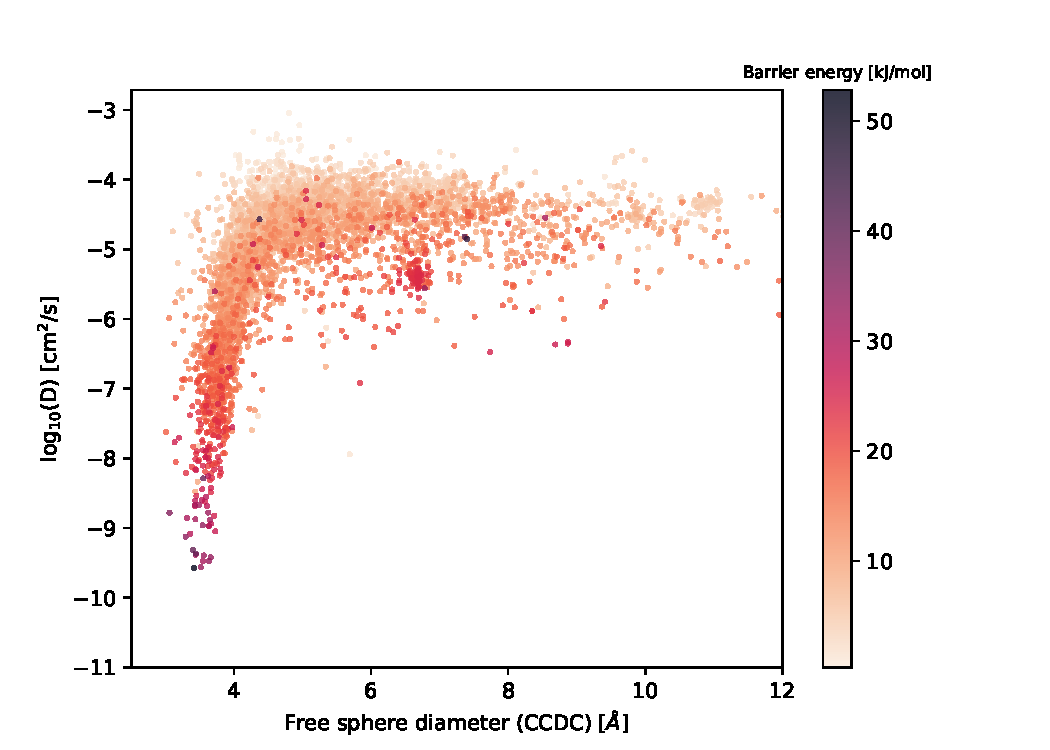
\includegraphics[width=0.48\textwidth]{figures/5-diffusion/difflog_Df-ccdc_barrier.pdf}
    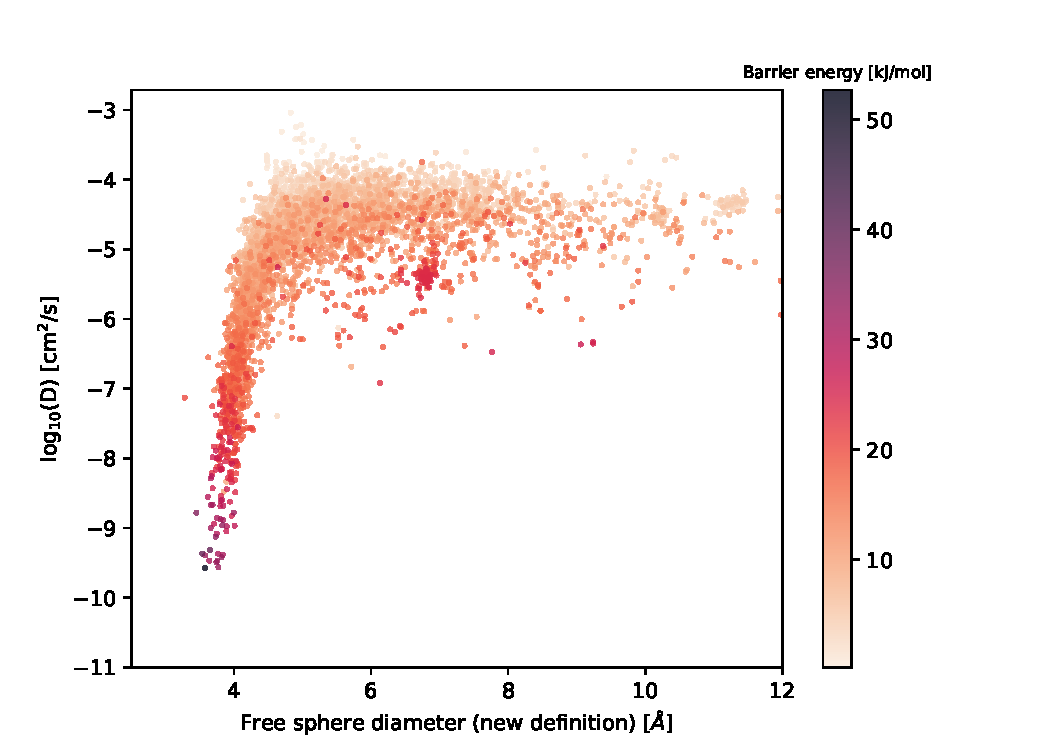
\includegraphics[width=0.48\textwidth]{figures/5-diffusion/difflog_Df-uff298K_barrier.pdf}
    \caption{\todo{correlation with PLD without labeling}}
    \label{fgr:}
\end{figure}

\subsection{Identification of interesting materials}

Outre l'exemple très parlant de SBMOF-1, d'autres publications, dans la séparation d'hydrocarbures notamment, s'intéressent aux éventuelles blocages cinétiques grâce à des simulations de dynamique moléculaire (MD) flexible.\cite{Stanton_2022} Ils ont notamment mis en évidence que la diffusion pouvait détériorer les performances de structure présentant d'excellente performance thermodynamique (énergie d'adsorption). Cette approche est très complète, car elle allie la thermodynamique, la flexibilité et les effets de transport dans une seule étude. En revanche, elle est très coûteuse en temps de calcul et ne pourrait être appliquée qu'à une poignée de structures. Au lieu d'utiliser des champs de force flexible qui alourdissent énormément la simulation, il est possible de se tourner vers une approche en ``snapshot'' bien moins coûteuse que nous développerons dans la dernière partie de ce rapport. Dans cette partie, nous nous focaliserons uniquement sur le couplage thermodynamique/cinétique.

Afin de recouper nos données purement structurelles et thermodynamiques avec des propriétés de transport, on a effectué un screening des coefficients de diffusion du xénon et du krypton sur les 7822 structures les plus sélectives. 
Des trajectoires de dynamique moléculaire ont été calculées sur l'ensemble de ces structures deux fois pour chaque adsorbat à dilution infinie. Il a fallu environ une à deux journées de simulation par structure afin de déterminer leurs coefficients de diffusion. Il est à noter pour la suite que les valeurs de diffusivités sont déterminés à l'ordre de grandeur près. Autrement dit c'est l'échelle logarithmique qui est pertinent pour les comparer à d'autres grandeurs. On a pu établir une forte corrélation entre le coefficient de diffusion et la taille minimale des canaux de diffusion à l'intérieur du matériau (PLD). La figure~\ref{fgr:Diff_Df_s} met en évidence la corrélation linéaire entre le logarithme de la diffusivité et le LCD pour des canaux de taille inférieure au diamètre cinétique du xénon (\SI{4,3}{\angstrom}). Ensuite, on arrive sur un plateau, c'est-à-dire que la diffusion du xénon dans le matériau ou dans le vide sont quasiment équivalentes. Les canaux sont assez larges pour permettre la libre diffusion du xénon à l'intérieur de ces matériaux. On voit aussi que ces matériaux ont moins de chances d'être sélectifs (les points foncés sont plus rares). Cette corrélation ouvre la voie au développement de modèles statistiques pour prédire la diffusivité, ce qui a déjà été étudié par Daglar \emph{et al.} dans leur récente publication.\cite{Daglar_2022} Dans leur étude, pour l'hélium, le coefficient de corrélation entre les coefficients de diffusion prédites et calculés par MD est d'environ 0,65 pour les données de test, ce qui n'est pas très précis. Il faut donc nuancer l'approche ``machine learning'' pour la prédiction des diffusivités. Cependant, l'étude n'a pas encore été menée sur le xénon et le krypton, ce qui pourrait mériter une étude préliminaire.

\begin{figure*}[t]
\centering
  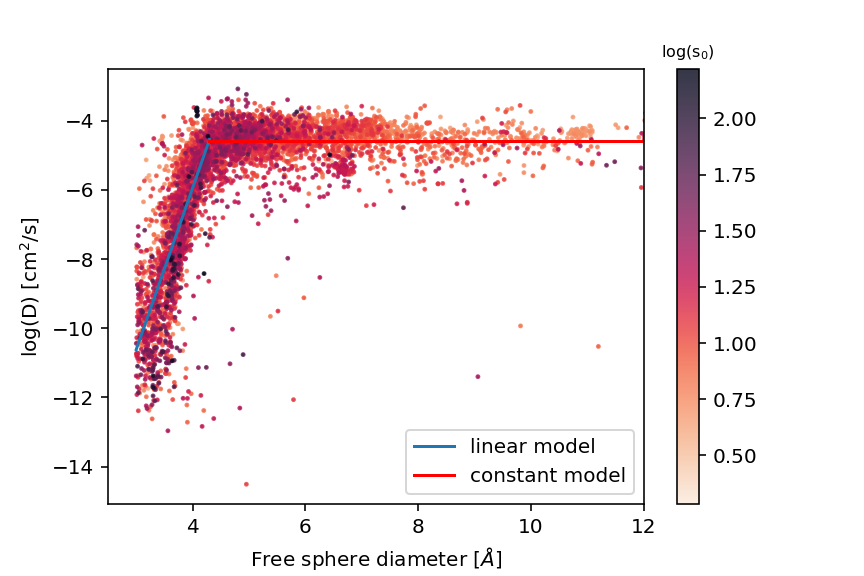
\includegraphics[width=0.8\textwidth]{figures/5-diffusion/D_log-diameter_colored_s_models+.png}
  \caption{\small{\ Logarithme du coefficient de diffusion du xénon à la limite des basses pressions en fonction du diamètre de la plus petite sphère libre dans le matériau (LCD). Les points sont colorés en fonction du logarithme de la sélectivité à basse pression $\log(s_0)$.}}
  \label{fgr:Diff_Df_s}
\end{figure*}

En analysant les rapports des coefficients de diffusion en comparaison des sélectivités, on a pu identifier deux structures qui couplent une bonne sélectivité à un ratio de diffusivités autour de 0,5 (\emph{cf.} table~\ref{table:diff}) : les structures de code CCSD GUMDEZ et QOZDOY. Grâce à leur LCD proches du diamètre cinétique du xénon et à un PLD assez élevé pour ne pas entraver le déplacement du xénon à travers les canaux. Les coefficients de diffusion du xénon tournent autour de 7$\times$10\ex{-5} \SI{}{\square\centi\meter\per\second} ce qui est proche de la diffusion libre (de l'ordre de 10\ex{-5} \SI{}{\square\centi\meter\per\second}), ce qui confirme l'absence de blocage cinétique. 

Une autre structure, ADOGEH (\emph{cf.} table~\ref{table:diff}), présente une diffusion 14 fois plus rapide pour le xénon que le krypton, tout en ayant une sélectivité à basse pression de 49. Ce phénomène s'explique par le fait que la structure a des canaux dans les trois directions et que pour changer de direction il faut passer par un canal plus étroit non accessible par le xénon. Ainsi le xénon, n'ayant qu'une direction de diffusion à l'intérieur du matériau, va bien plus vite que le krypton pour lequel toutes les directions s'offrent à lui. Ainsi, le krypton est plus lent à diffuser car il change de direction constamment dans le matériau contrairement au xénon. En revanche, la sélectivité baisse à 10 lorsque l'on considère un mélange de 20/80 Xe/Kr à pression ambiante au lieu de la dilution infinie. Ce matériau pourrait être utile notamment à pression partielle faible en xénon et krypton, ce qui est le cas pour notre application. Des études plus approfondies sont encore à mener, notamment en confirmant les valeurs de sélectivité par des calculs DFT plus fiable ou en étudiant la flexibilité ; mais si les résultats sont concluant ces matériaux pourraient alors être testés expérimentalement pour une éventuelle application industrielle.

\begin{table}[t]
\centering
\begin{tabular}{|l|r|r|r|r|r|r|}
\hline
  CCSD ref. code &      LCD (\SI{}{\angstrom}) &    s$_1$ &       s$_0$ &     PLD (\SI{}{\angstrom}) &     Ratio Diff. &  Coeff. de Diff. Xe \\
\hline
QOZDOY\cite{Zhang_2001} &  5,3 & 37 & 52 & 4,7 &  0.4 &               7$\times$10\ex{-5} \SI{}{\square\centi\meter\per\second} \\
GUMDEZ\cite{Yin_2014} &  5,3 & 42 & 56 & 4,8 &  0.5 &               7$\times$10\ex{-5} \SI{}{\square\centi\meter\per\second} \\
ADOGEH\cite{Peikert_2012} & 12,7 &  10 & 49 & 5,1 & 14 &               5$\times$10\ex{-5} \SI{}{\square\centi\meter\per\second} \\
\hline
\end{tabular}
\caption{\ Performances de structures identifiées par un screening prenant en compte les coefficients de diffusion. }
\label{table:diff}
\end{table}

Les résultats d'un screening couplant thermodynamique et cinétique permettent déjà de mettre en valeur des matériaux encore inconnus de la communauté. La question du blocage cinétique est certes traitée dans certaines études,\cite{Stanton_2022} mais aucune approche systématique n'a encore été développée. Ces structures ont des sélectivités élevées mais ne sont pas les plus sélectives; elles auraient donc été écartées dans un screening standard basé uniquement sur la thermodynamique. 

Cette approche basée sur des trajectoires de dynamique moléculaire présente toutefois ses propres défauts. En effet, la méthode est très lente (quelques jours de simulation par structure), les structures avec différents canaux non connectées posent problème car l'adsorbat ne peut diffuser que dans un seul des deux canaux. Ainsi, il faudrait dans certains cas faire plusieurs trajectoires ce qui demande encore davantage de temps de calcul. De plus, si l'on veut ajouter de la flexibilité, cette méthode ne pourrait être utilisée que sur quelques structures. C'est pourquoi, un algorithme bien plus efficace est en cours d'implémentation en C++ pour accélérer les calculs de diffusivité. Un tel algorithme est déjà conçu par le groupe de Berend Smit à l'EPFL \cite{Mace_2019}, mais le code étant sous Matlab (langage peut efficace), il est impossible de l'utiliser dans des procédures de screening. Cet algorithme détermine des sites d'adsorption et des états de transition pour passer d'un site à un autre. Puis à l'aide de simulations de Monte Carlo cinétique l'adsorbat se déplace d'un site à un autre au rythme d'une constante cinétique déterminée par l'état de transition. Cette méthode permet également d'identifier en avance les différents canaux et on assure que chacun d'entre eux sont traversés par des molécules. Par conséquent, ce nouveau code permettrait de résoudre les problèmes de temps de calcul et de fiabilité rencontrés avec la dynamique moléculaire. 

\section{Fast diffusion calculation algorithm}

\subsection{Implementation in C++}

\subsection{Preliminary results}

\subsection{Visualization tool}

\todo{Take some examples for the vizualisation with comparison to the pore size and diffusion coefficient}

\subsection{Development of a first prediction model}

\begin{figure}[ht]
  \centering
    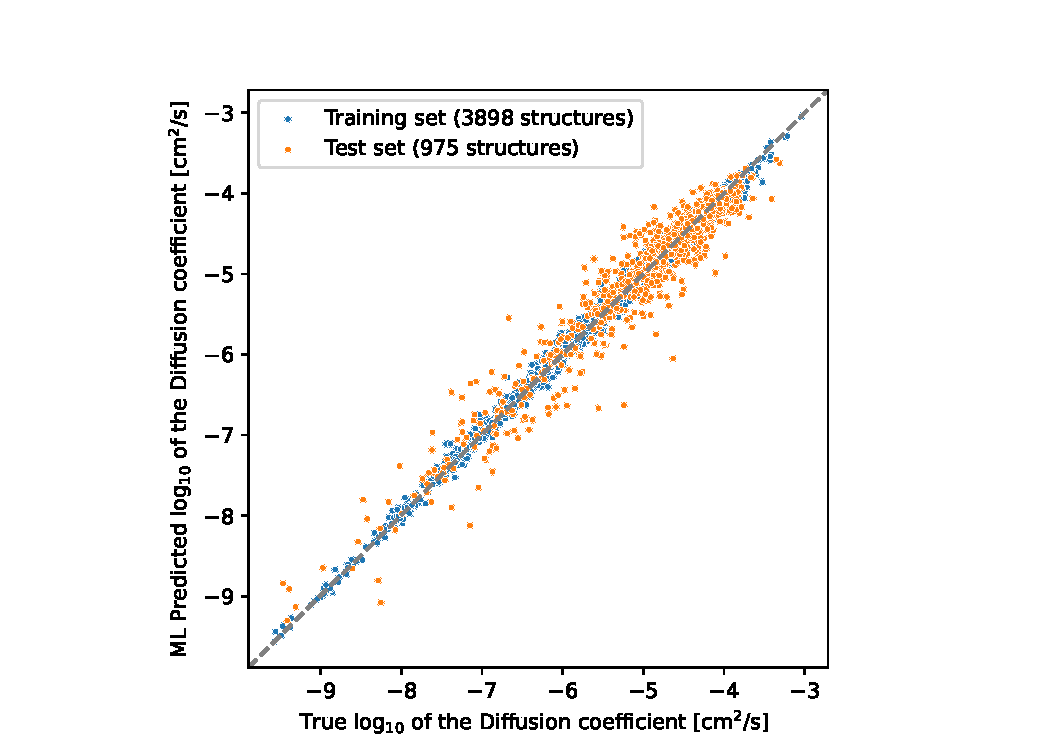
\includegraphics[width=6cm]{figures/5-diffusion/diffusion_prediction.pdf}
    \caption{}
    \label{fgr:}
\end{figure}

\begin{figure}[ht]
  \centering
    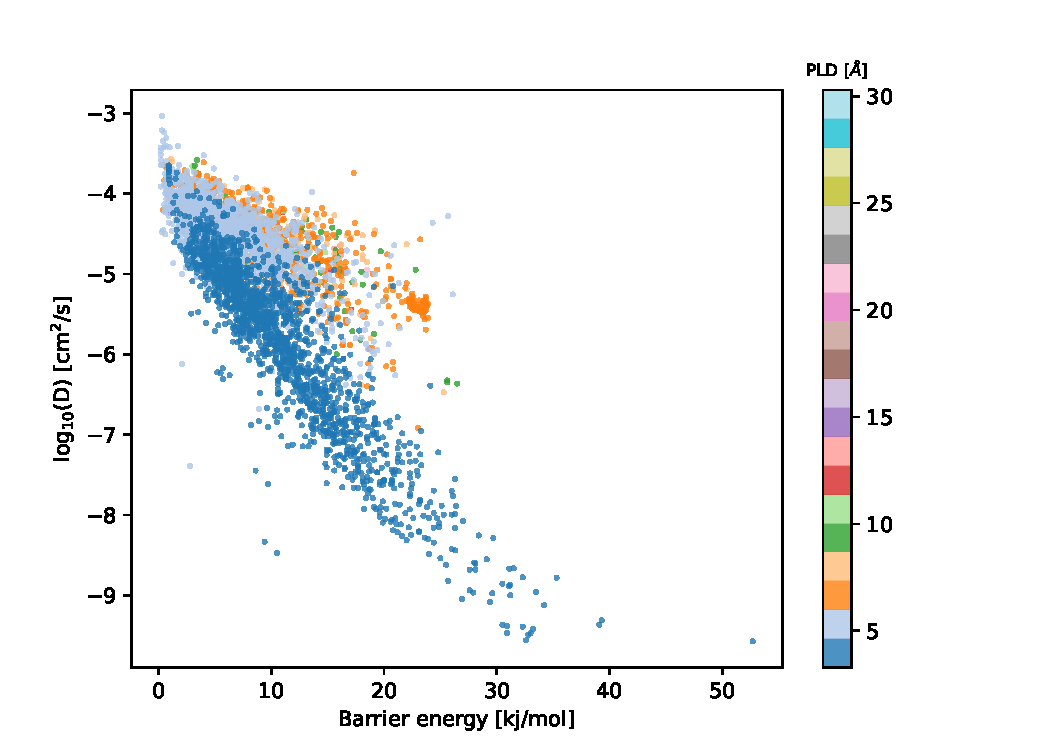
\includegraphics[width=0.48\textwidth]{figures/5-diffusion/difflog_barrier_Df_uff.pdf}
    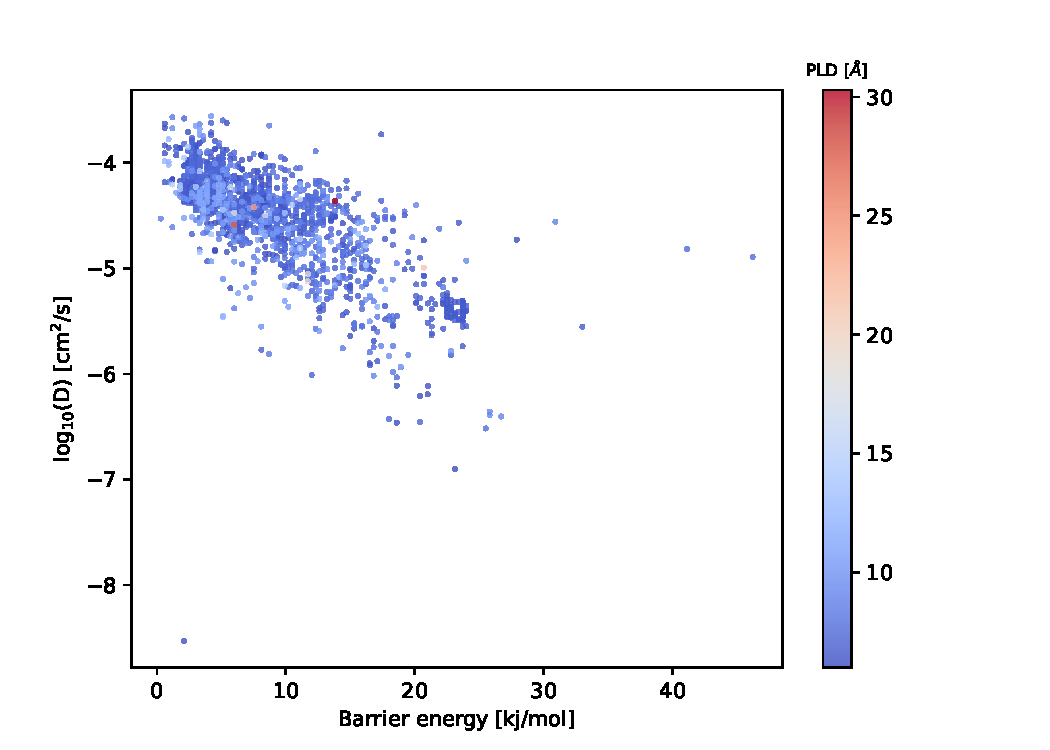
\includegraphics[width=0.48\textwidth]{figures/5-diffusion/difflog_barrier_Df_uff_2.pdf}
    \caption{}\label{fgr:}
\end{figure}

\begin{figure}[ht]
  \centering
    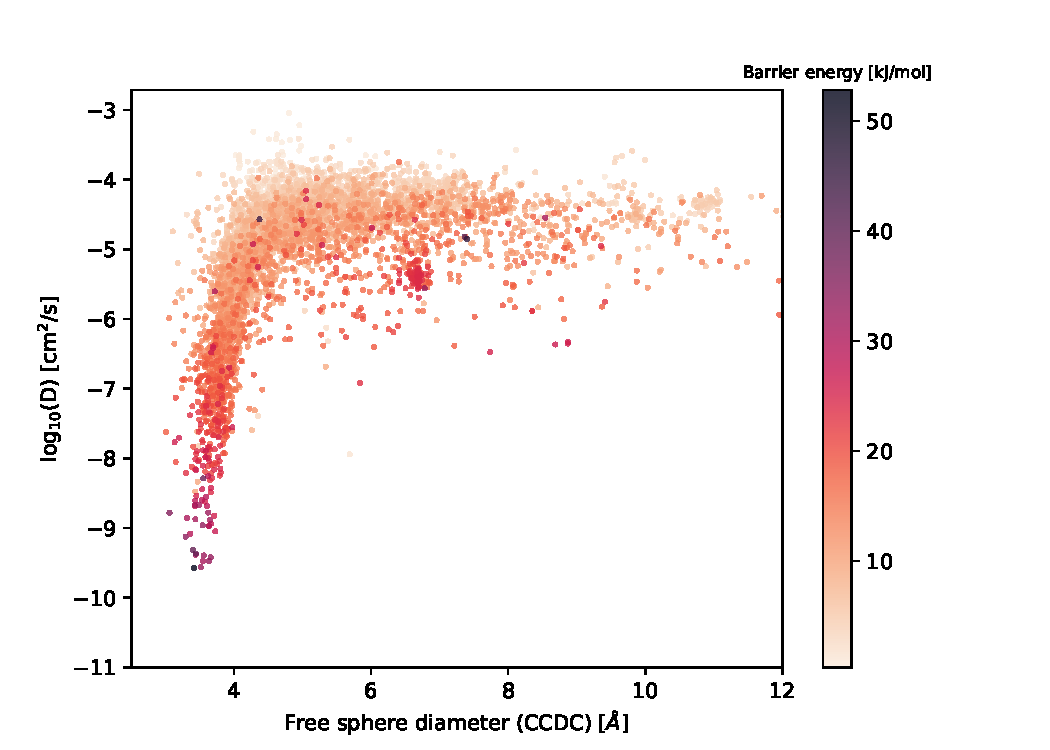
\includegraphics[width=0.48\textwidth]{figures/5-diffusion/difflog_Df-ccdc_barrier.pdf}
    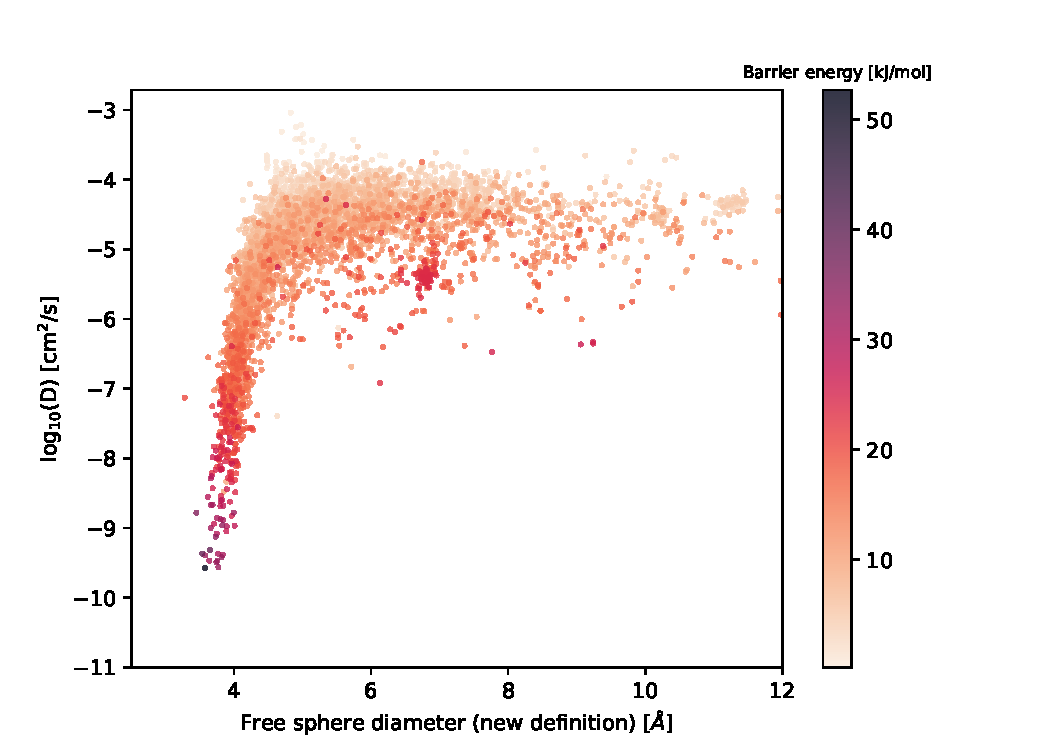
\includegraphics[width=0.48\textwidth]{figures/5-diffusion/difflog_Df-uff298K_barrier.pdf}
    \caption{}
    \label{fgr:}
\end{figure}

ML descriptors
next steps

\OnlyInSubfile{\printglobalbibliography}

\end{document}
